\section{Sum of Exterior Angles of a Polygon}

The sum of the exterior angles of a polygon is \(360^{\circ}\)
\[Sum_{ext} = 360^{\circ}\]
\\
As long as the polygon has no concavity to its shape.

\subsection{Conjecture}

By definition, all the angles in a circle sum up to be \(360^{\circ}\) \\
\[\sum\limits_{n=1}^{N}{a_n} = 360^{\circ}\] \\

\begin{center}
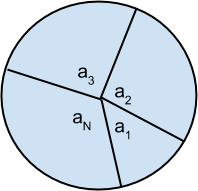
\includegraphics[width=8cm]{Geometry/polygon_ext_angles_diag1}
\end{center}
The lines can be extended and removed from the center, while still keeping their orientation. \\
\begin{center}
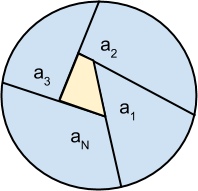
\includegraphics[width=8cm]{Geometry/polygon_ext_angles_diag2}
\end{center}
The relative angles, \(a_n\), between each line remains the same, and a polygon is formed in the middle.\\
\\
This is only true for polygons that can be created using this method.  A polygon like the one below is impossible to create using this method. \\
\\
\begin{center}
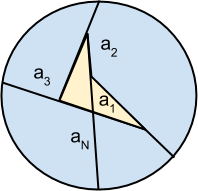
\includegraphics[width=8cm]{Geometry/polygon_ext_angles_diag3}
\end{center}
Hence, \(Sum_{ext} = 360^{\circ}\) is true only for polygons with no concavity \\
\\

\section{Sum of Interior Angles of a Polygon}
The sum of the interior angles of a polygon is
\[Sum_{ing} = (N-2)180^{\circ}\] \\
where N is the number of sides of the polygon\\
\\
As long as the polygon has no concavity to its shape.\\
\\
\subsection{Derivation}

The sum of all the exterior angles is 
\[\sum\limits_{n=1}^{N}{a_n} = 360^{\circ}\] \\
\\
Exterior and interior angles are the compliments of each other.  So if \(a_n\) is the exterior angle, then \(180-a_n\) is the interior angle and \\

\begin{align*}
Sum_{int} &= \sum\limits_{i=1}^N{180^{\circ}-a_n}\\
&= 180^{\circ}\sum\limits_{i=1}^N{1}-\sum\limits_{i=1}^N{a_n}\\
&= 180^{\circ}\sum\limits_{i=1}^N{1}-360^{\circ}\\
&= 180^{\circ}N-360^{\circ}\\
Sum_{int} &= (N-2)180^{\circ}
\end{align*}
\\

\section{Area of a Rectangle}

\section{Area of a Triangle}

\subsection{Derivation: $\frac{1}{2}bh$}

\subsection{Derivation: Heron's formula}

\section{Area of a Circle}

The area of a circle is most commonly stated as

\[A = \pi r^2\]
\\
where \(r\) is the radius of the circle

\subsection{Derivation: Cartesian coordinates}

\subsection{Derivation: Polar coordinates}
The easiest derivation of the area of a circle is to simply use polar coordinates where the differential volume is 
\[dv = rd\theta dr\]

\begin{align*}
A =& \oint dv \\
A =& \int\limits_{0}^{2\pi}\int\limits_{0}^{r} rd\theta dr \\
A =& \bigg[ \theta \bigg|_{0}^{2\pi}\bigg[ \frac{1}{2}r^2 \bigg|_{0}^{r} \\
A =& [2\pi - 0]\frac{1}{2}[r-0] \\
A =& \pi r^2
\end{align*}
\\
\subsection{Conjecture: No Calculus}

Inscribe an N-sided polygon in a circle or radius \(R\).  Each interior angle will be \(\theta =\frac{2\pi}{N}\).  The polygon will be made up of \(N\) triangles.  Each of these triangles will have an area of
\[A_{triangle} = \frac{bh}{2} = \frac{R\cos(\frac{\theta}{2})2R\sin(\frac{\theta}{2})}{2}\]
And the area of the polygon will be
\begin{align*}
A_{poly} =& NR\cos(\frac{\theta}{2})R\sin(\frac{\theta}{2})\\
A_{poly} =& R^2N\cos(\frac{\pi}{N})\sin(\frac{\pi}{N})\\
\end{align*}
What happens when you increase \(N\) larger and larger and large?  What happens when \(N\) approaches infinity\\
\\
We can use the approximations\\
\(\sin(\alpha) \approx \alpha\), for really small \(\alpha\)\\
and of course\\
\(\\cos(0) = 1\)\\
\\
So
\begin{align*}
A_{poly} =& A_{circ} = R^2\cos(\frac{\pi}{N})N\sin(\frac{\pi}{N})\\
A_{poly} =& A_{circ} = R^2(1))(N\frac{\pi}{N}))\\
A_{circ} =& \pi R^2
\end{align*}

\section{Volume of a Sphere}

\section{Surface Area of a Cone}